\documentclass[a4paper]{article}
\usepackage[utf8x]{inputenc}
\usepackage[T1,T2A]{fontenc}
\usepackage[russian]{babel}
\usepackage{hyperref}
\usepackage{indentfirst}
\usepackage{color}
\usepackage{listings}
\usepackage{here}
\usepackage{array}
\usepackage{multirow}
\usepackage{graphicx}
\usepackage{caption}

\lstset{ %
extendedchars=\true,
keepspaces=true,
language=C++,					% choose the language of the code
basicstyle=\footnotesize,		% the size of the fonts that are used for the code
numbers=left,					% where to put the line-numbers
numberstyle=\footnotesize,		% the size of the fonts that are used for the line-numbers
stepnumber=1,					% the step between two line-numbers. If it is 1 each line will be numbered
numbersep=5pt,					% how far the line-numbers are from the code
backgroundcolor=\color{white},	% choose the background color. You must add \usepackage{color}
showspaces=false				% show spaces adding particular underscores
showstringspaces=false,			% underline spaces within strings
showtabs=false,					% show tabs within strings adding particular underscores
frame=single,           		% adds a frame around the code
tabsize=4,						% sets default tabsize to 2 spaces
captionpos=b,					% sets the caption-position to bottom
breaklines=true,				% sets automatic line breaking
breakatwhitespace=false,		% sets if automatic breaks should only happen at whitespace
escapeinside={\%*}{*)},			% if you want to add a comment within your code
postbreak=\raisebox{0ex}[0ex][0ex]{\ensuremath{\color{red}\hookrightarrow\space}}
}
\begin{document}	% начало документа


\begin{titlepage}	% начало титульной страницы

	\begin{center}		% выравнивание по центру

		\large Санкт-Петербургский Политехнический Университет Петра Великого\\
		\large Институт компьютерных наук и технологий \\
		\large Кафедра компьютерных систем и программных технологий\\[6cm]
		% название института, затем отступ 6см
		
		\huge Программирование\\[0.5cm] % название работы, затем отступ 0,5см
		\large Отчет по курсовой работе\\[0.1cm]
		\large Модель "Хищник - жертва"\\[5cm]

	\end{center}


	\begin{flushright} % выравнивание по правому краю
		\begin{minipage}{0.25\textwidth} % врезка в половину ширины текста
			\begin{flushleft} % выровнять её содержимое по левому краю

				\large\textbf{Работу выполнил:}\\
				\large Жуйков А.А.\\
				\large {Группа:} 13501/4\\
				
				\large \textbf{Преподаватель:}\\
				\large Вылегжанина К.Д.
				

			\end{flushleft}
		\end{minipage}
	\end{flushright}
	
	\vfill % заполнить всё доступное ниже пространство

	\begin{center}
	\large Санкт-Петербург\\
	\large \the\year % вывести дату
	\end{center} % закончить выравнивание по центру

\thispagestyle{empty} % не нумеровать страницу
\end{titlepage} % конец титульной страницы

\vfill % заполнить всё доступное ниже пространство
% Содержание
\tableofcontents
\newpage

\section{Модель Хищник-жертва}
\subsection{Задание}
На прямоугольном поле случайным образом размещаются "хищники" и "жертвы", после чего они поочередно делают ходы. Ход жертвы - случайное перемещение на соседнюю клетку, раз в несколько ходов жертва порождает еще одну жертву на соседней клетке. Ход хищника - уничтожение жертвы на соседней клетке, если это возможно, иначе - случайное перемещение на соседнюю клетку. Уничтожив несколько жертв, хищник порождает еще одного хищника на соседней клетке. Оставшись без еды на несколько ходов, хищник умирает. Реализовать на экране процесс борьбы хищников и жертв. 

\subsection{Концепция}
На прямоугольном поле случайным образом размещаются "хищники" и "жертвы", после чего они поочередно делают ходы. Ход жертвы - случайное перемещение на соседнюю клетку. Раз в несколько ходов жертва порождает еще одну жертву на соседней клетке, если у нее достаточно энергии. Чтобы выжить и получить энергию, жертве неоходимо питаться. На случайной клетке поля "вырастают" растения - пища для жертвы. Ход хищника - уничтожение жертвы на соседней клетке, если это возможно, иначе - случайное перемещение на соседнюю клетку. Уничтожив несколько жертв, хищник порождает еще одного хищника на соседней клетке. Оставшись без еды на несколько ходов, хищник умирает. Реализовать на экране процесс борьбы хищников и жертв. 

\subsection{Диаграмма прецедентов использования}
На рис \ref{pic:UseCaseDiagram1} показана диаграмма прецедентов использования.
\begin{figure}[H]
	\begin{center}
		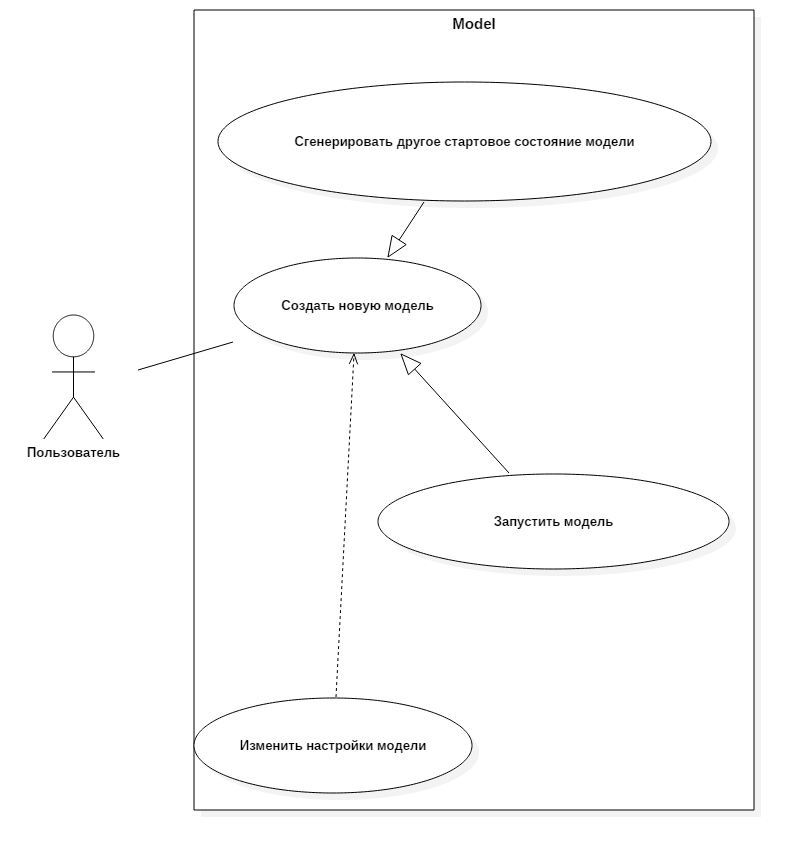
\includegraphics[scale=0.4, height=7cm]{pictures/UseCaseDiagram}
		\caption{Диаграмма прецедентов использования} 
		\label{pic:UseCaseDiagram1} % название для ссылок внутри кода
	\end{center}
\end{figure}

\subsection{Вывод}
Определены правила модели. Составлена диаграмма прецедентов использования.
\section{Проектрование приложения, реализующего модель Хищник-жертва}
Приложение позволяет задавать следующие настройки модели: начальные количества хищников и жертв, длина и высота поля, количество ходов хищника без еды. 

\begin{figure}[H]
	\begin{center}
		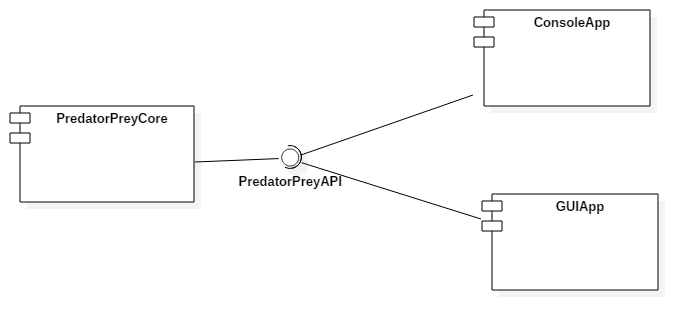
\includegraphics[scale=0.4, height=7cm]{pictures/ComponentDiagram1}
		\caption{Диаграмма прецедентов использования} 
		\label{pic:ComponentDiagram} % название для ссылок внутри кода
	\end{center}
\end{figure}

\subsection{Библиотека}
Библиотека  - ядро приложения. Здесь содержатся основные классы, необходимые для представления модели. 

\noindent В API выделены следующие методы: 
\begin{itemize}
\item Метод, создающий хищников на поле, количество которых задано в настройках.
\item Метод, создающий жертв на поле, количество которых задано в настройках.
\item Методы, удаляющие умерших хищников и жертв в конце хода.
\item Методы, передвигающие всех хищников и жертв на поле.
\item Метод, возвращающий true, если хищники или жертвы исчезли с поля и false в обратном случае.
\item Методы, возвращающие текущее количество хищников и жертв на поле.
\item Методы, возвращающие текущие день и время модели, необходимые для подсчета времени существования модели. 
8. Метод, возвращающий указатель на поле модели. 
\end{itemize}

\subsection{Вывод}
Было решено, какие настройки возможно изменить в модели. Выделены основные методы API. 

\section{Реализация модели Хищник - жертва}
\subsection{Среда разработки}
\noindent Операционная система Windows 8.1

\noindent Интегрированная среда разработки Qt Creator 3.6.1

\noindent Стандарт C++, C++11

\noindent Компилятор MinGW 4.9.2 

\noindent Система документирования Doxygen 1.8.8

\noindent Утилита для статического анализа кода Cppcheck 1.67

\subsection{Консольное приложение}
Консольное приложение предоставляет пользователю всю функциональность ядра и позволяет работать с моделью в консоли. 

\noindent Основные классы, выделенные в консольном приложении:
\begin{itemize}
\item Класс ConsoleApp. Создает модель, настройки модели, организует консольное взаимодействие с пользователем. Здесь же задается промежуток времени для вывода состояния модели.
\item Класс ConsoleDialog. Содержит консольные меню для взаимодействия с пользователем: меню настроек, главное меню. Реализована обработка неверного ввода. 
\item Класс ConsoleDrawer. Выводит в консоль состояние модели, а также другую информацию: количество хищников и жертв на поле, время и день модели, легенду. 
\end{itemize}

На рис \ref{pic:consoleMain} представлено главное меню приложения. Есть возможность начать новую модель, изменить ее настройки и выйти из приложения. 

\begin{figure}[H]
	\begin{center}
		\includegraphics[scale=0.5]{consoleMain}
		\caption{Главное меню консольного приложения} 
		\label{pic:consoleMain} % название для ссылок внутри кода
	\end{center}
\end{figure}

На рис \ref{pic:consoleSettings} показано меню настроек с возможностью выбора, что изменить. Справа от настройки отображается ее текущее состояние.

\begin{figure}[H]
	\begin{center}
		\includegraphics[scale=0.5]{consoleSettings}
		\caption{Настройки модели в консольном приложении} 
		\label{pic:consoleSettings} % название для ссылок внутри кода
	\end{center}
\end{figure}

На рис \ref{pic:consoleField} – поле модели с находящимися на нем хищниками и жертвами. Над полем выводится легенда и текущее количество агентов. 

\begin{figure}[H]
	\begin{center}
		\includegraphics[scale=0.5]{consoleField}
		\caption{Поле модели в консольном приложении} 
		\label{pic:consoleField} % название для ссылок внутри кода
	\end{center}
\end{figure}

\subsection{Библиотека}
\noindent Основные классы, выделенные в библиотеке:
\begin{itemize}
\item Класс Model. Реализует методы, заявленные  в API. Содержит поле модели, класс с векторами хищников и жертв, текущие время и день, а также указатель на используемые настройки.
\item Класс Settings. Содержит настройки модели: высота и длина поля, количество хищников и жертв на поле, время жизни хищника без еды и другие. 
\item Класс Field. Класс представляет поле модели. Реализуется в виде вектора векторов позиций поля (enum class Position). Присутствуют методы, возвращающие высоту и длину поля, статус указанной клетки, свободное направление для указанной клетки. В классе определены целочисленные константы, в которых записаны максимальный и минимальный размеры поля. 
\item Класс Units. Содержит вектора указателей на хищников и жертв.
\item Класс Animal – базовый класс для классов хищников и жертв. Содержит поля, необходимые для представления агентов: время нахождения на поле, энергия, направление для следующего хода, указатель на поле и другие. А также общие методы: метод выбора направления следующего хода, метод перемещения агента по текущему направлению,  метод выбора случайного направления и другие. 
\item Класс Predator представляет хищника в модели. Класс реализует полиморфные методы класса Animal и добавляет новые методы и поля к базовому классу: метод уничтожающий жертву, метод поиска жертвы, метод создающий нового хищника, метод передвигающий хищника. Также содержит поля: указатель на жертву – текущая цель, указатель на Units.
\item Класс Prey представляет жертву в модели. Как и в классе Predator, здесь присутствует реализация полиморфных методов из класса Animal. 
\end{itemize}

\subsection{Графическое приложение}
На рис \ref{pic:FOX} представлено главное окно приложения. Пользователю, как и в консольном приложении, предоставляется возможность начать новую модель, изменить ее настройки и выйти. 

\begin{figure}[H]
	\begin{center}
		\includegraphics[scale=0.5]{FOX}
		\caption{Главное меню графического приложения} 
		\label{pic:FOX} % название для ссылок внутри кода
	\end{center}
\end{figure}

На рис \ref{pic:GUIsettings} – окно настроек приложения. Все начальные параметры модели можно изменить, после чего сохранить изменения. Если выйти из настроек, не нажав на кнопку «сохранить», то настройки не изменятся.

\begin{figure}[H]
	\begin{center}
		\includegraphics[scale=0.5]{GUIsettings}
		\caption{Настройки модели в графическом приложении} 
		\label{pic:GUIsettings} % название для ссылок внутри кода
	\end{center}
\end{figure}

Состояние поля модели, и его текущее состояние представлены на рис \ref{pic:GUImain} 

\begin{figure}[H]
	\begin{center}
		\includegraphics[scale=0.5]{GUImain}
		\caption{Представление модели в графическом приложении} 
		\label{pic:GUImain} % название для ссылок внутри кода
	\end{center}
\end{figure}

\noindent Основные классы, выделенные в графическом приложении. 
\begin{itemize}
\item Класс MainMenu. Главное окно приложения. Присутствуют кнопки «Новая модель», «Настройки», «Выход». При попытке выхода появляется окно подтверждения. 
\item Класс SettingsWindow. Окно для изменения настроек модели. Можно выйти как без сохранения настроек, так и с сохранением. 
\item Класс ModelWindow. Окно для представления модели. Содержит фрейм поля, в котором выводится состояние поля на каждом шаге моделирования, и фрейм статуса модели, где содержится информация о текущем состоянии модели. Также присутствуют кнопки «Старт», «Сгенерировать», «Выйти в меню».  
\end{itemize}

\subsection{Вывод}
Для реализации модели определены основные классы ядра, консольного и графического приложений. Разделение на подпроекты упрощает процесс работы над проектом.
\section{Процесс обеспечения качества и тестирование}
\subsection{Просмотр кода}
В ходе проектирования дважды была проведена проверка исходного кода программы с целью обнаружения и исправления ошибок (code review). В результате было получено около 80-ти замечаний в каждом.

Большая часть замечаний исправлена. 
\subsection{Демонстрации}
Всего было проведено три демонтрации:
\begin{itemize}

\item Демонстрация №1.
Отрисовка модели в консоль, изменение настроек.

Замечания:

\begin{itemize}
\item Сделать один язык во всем приложении. 
\item Исправить время модели, создающейся с новыми параметрами.
\end{itemize}

\item Демонстрация №2.
Движение, порождение/исчезновение хищников.

Замечания:

\begin{itemize}
\item Непонятные фразы результата моделирования: "Хищники победили", "Жертвы победили".
\end{itemize}

\item Демонтрация №3.
Последняя демонтрация перед релизом консольного приложения

Замечания:

\begin{itemize}
\item Не выходить из меню настроек после их изменения.
\item Добавить обработку ввода.
\item Добавить легенду
\item Выводить текущую статистику
\end{itemize}

\end{itemize} 
Все недочеты исправлены, учтены пожелания других участников демонстраций. 

\subsection{Непрерывная интеграция}
Непрерывная интеграция была осуществлена при помощи приложения jenkins, установленного на сервере с операционной системой Ubuntu. На сервере код приложения проверялся следующими и другими утилитами, строились графики: 

Cppcheck – утилита для статического анализа кода. Благодаря ей были найдены и исправлены многие стилистические ошибки. 

Valgrind – утилита для обнаружения утечек памяти. С ее помощью быстро исправлялись ошибки в работе с памятью.

Gcov – утилита, которая считает процент покрытия кода тестами. Во время работы процент повысился до 70%. 
\subsection{Тестирование}
Приложение содержит модульные тесты. Протестированы некоторые основные классы. Имеется большое количество тестов класса Predator: проверяется правильность нахождения направления к жертве, порождение, движение, исчезновение хищника. В ходе работы над проектом покрытие тестами не опускалось ниже 40%. 

\subsection{Вывод}
Тестирование приложения - важная часть разработки. Созданные тесты помогали быстро определить ошибку.
\section{Вывод}
Курсовая работа этого семестра – это отличная возможность ближе познакомиться с языком, глубже его понять. Проведенные семинары по эффективному использованию STL, новым стандартам языка программирования подкрепляют полученные знания и открывают новые возможности использования средств языка. 

Работа над приложением будет продолжаться. Планируется добавить еду для жертв;  новые тесты, привести в порядок имеющиеся. Хищники должны ускоряться во время преследования жертвы, при этом тратить энергию. Возможно, в процессе улучшения появятся новые идеи для оптимизации алгоритмов ярда. 

Таким образом, во время работы над проектом, автор приобрел большой практический опыт в области объектно-ориентированного проектирования на языке C++. 

\section{Приложение 1. Листинги кода}
\subsection{Библиотека}
\lstinputlisting[]
{../sources/Predator-prey/lib/modelapi.h}
\newpage

\lstinputlisting[]
{../sources/Predator-prey/lib/model.h}
\lstinputlisting[]
{../sources/Predator-prey/lib/model.cpp}
\newpage

\lstinputlisting[]
{../sources/Predator-prey/lib/animal.h}
\lstinputlisting[]
{../sources/Predator-prey/lib/animal.cpp}
\newpage

\lstinputlisting[]
{../sources/Predator-prey/lib/field.h}
\lstinputlisting[]
{../sources/Predator-prey/lib/field.cpp}
\newpage

\lstinputlisting[]
{../sources/Predator-prey/lib/settings.h}
\lstinputlisting[]
{../sources/Predator-prey/lib/settings.cpp}
\newpage

\lstinputlisting[]
{../sources/Predator-prey/lib/units.h}
\lstinputlisting[]
{../sources/Predator-prey/lib/units.cpp}
\newpage

\lstinputlisting[]
{../sources/Predator-prey/lib/animal.h}
\lstinputlisting[]
{../sources/Predator-prey/lib/animal.cpp}
\newpage

\lstinputlisting[]
{../sources/Predator-prey/lib/predator.h}
\lstinputlisting[]
{../sources/Predator-prey/lib/predator.cpp}
\newpage

\lstinputlisting[]
{../sources/Predator-prey/lib/prey.h}
\lstinputlisting[]
{../sources/Predator-prey/lib/prey.cpp}
\newpage

\lstinputlisting[]
{../sources/Predator-prey/lib/coordinates.h}
\lstinputlisting[]
{../sources/Predator-prey/lib/coordinates.cpp}
\newpage

\lstinputlisting[]
{../sources/Predator-prey/lib/badboundary.h}
\lstinputlisting[]
{../sources/Predator-prey/lib/badnum.h}
\lstinputlisting[]
{../sources/Predator-prey/lib/badfield.h}
\newpage

\subsection{Консольное приложение}

\lstinputlisting[]
{../sources/Predator-prey/consoleApp/main.cpp}
\newpage

\lstinputlisting[]
{../sources/Predator-prey/consoleApp/consoleapp.h}
\lstinputlisting[]
{../sources/Predator-prey/consoleApp/consoleapp.cpp}
\newpage

\lstinputlisting[]
{../sources/Predator-prey/consoleApp/consoledialog.h}
\lstinputlisting[]
{../sources/Predator-prey/consoleApp/consoledialog.cpp}
\newpage

\lstinputlisting[]
{../sources/Predator-prey/consoleApp/consoledrawer.h}
\lstinputlisting[]
{../sources/Predator-prey/consoleApp/consoledrawer.cpp}

\lstinputlisting[]
{../sources/Predator-prey/consoleApp/badinput.h}
\newpage

\subsection{Графическое приложение}

\lstinputlisting[]
{../sources/Predator-prey/GUIApp/main.cpp}

\lstinputlisting[]
{../sources/Predator-prey/GUIApp/modelgui.h}
\lstinputlisting[]
{../sources/Predator-prey/GUIApp/modelgui.cpp}
\newpage

\lstinputlisting[]
{../sources/Predator-prey/GUIApp/mainmenu.h}
\lstinputlisting[]
{../sources/Predator-prey/GUIApp/mainmenu.cpp}
\newpage

\lstinputlisting[]
{../sources/Predator-prey/GUIApp/modelwindow.h}
\lstinputlisting[]
{../sources/Predator-prey/GUIApp/modelwindow.cpp}
\newpage

\lstinputlisting[]
{../sources/Predator-prey/GUIApp/settingswindow.h}
\lstinputlisting[]
{../sources/Predator-prey/GUIApp/settingswindow.cpp}
\newpage

\lstinputlisting[]
{../sources/Predator-prey/GUIApp/exitwindow.h}
\lstinputlisting[]
{../sources/Predator-prey/GUIApp/exitwindow.cpp}
\newpage

\lstinputlisting[]
{../sources/Predator-prey/GUIApp/fieldframe.h}
\lstinputlisting[]
{../sources/Predator-prey/GUIApp/fieldframe.cpp}
\newpage

\lstinputlisting[]
{../sources/Predator-prey/GUIApp/statusframe.h}
\lstinputlisting[]
{../sources/Predator-prey/GUIApp/statusframe.cpp}
\newpage

\lstinputlisting[]
{../sources/Predator-prey/GUIApp/resultwindow.h}
\lstinputlisting[]
{../sources/Predator-prey/GUIApp/resultwindow.cpp}

\subsection{Модульные тесты}

\lstinputlisting[]
{../sources/Predator-prey/tests/tst_modeltest.cpp}
\newpage
\end{document}